\documentclass[UTF8]{article}
\usepackage{graphicx}
\usepackage{subfigure}
\usepackage{amsmath}
\usepackage{makecell}
\usepackage[utf8]{inputenc}
\usepackage[space]{ctex} %中文包
\usepackage{listings} %放代码
\usepackage{xcolor} %代码着色宏包
\usepackage{CJK} %显示中文宏包
\usepackage{float}
\usepackage{makecell}
\usepackage{diagbox}
\usepackage{bm}
\usepackage{ulem} 
\usepackage{amssymb}
\usepackage{soul}
\usepackage{color}
\usepackage{geometry}
\usepackage{fancybox} %花里胡哨的盒子
\usepackage{xhfill} %填充包, 可画分割线 https://www.latexstudio.net/archives/8245
\usepackage{multicol} %多栏包
\usepackage{enumerate} %可以方便地自定义枚举标题
\usepackage{multirow} %表格中多行单元格合并
\usepackage{wasysym} %可以使用wasysym里的一堆奇奇怪怪的符号
\usepackage[marginal]{footmisc} % 注脚, 且不缩进

\geometry{left = 2.5cm, right = 2.5cm, bottom = 2.5cm, top = 2.5cm}

\definecolor{mygreen}{rgb}{0,0.6,0}
\definecolor{mygray}{rgb}{0.5,0.5,0.5}
\definecolor{mymauve}{rgb}{0.58,0,0.82}

\lstset{
	backgroundcolor=\color{white}, 
	%\tiny < \scriptsize < \footnotesize < \small < \normalsize < \large < \Large < \LARGE < \huge < \Huge
	basicstyle = \scriptsize,       
	breakatwhitespace = false,        
	breaklines = true,                 
	captionpos = b,                    
	commentstyle = \color{mygreen}\bfseries,
	escapeinside=``,
	extendedchars = false,
	frame = shadowbox, 
	framerule=0.5pt,
	keepspaces=true,
	keywordstyle=\color{blue}\bfseries, % keyword style
	language = verilog,                     % the language of code
	otherkeywords={string}, 
	numbers=left, 
	numbersep=5pt,
	numberstyle=\tiny\color{mygray},
	rulecolor=\color{black},         
	showspaces=false,  
	showstringspaces=false, 
	showtabs=false,    
	stepnumber=1,         
	stringstyle=\color{mymauve},        % string literal style
	tabsize=4,          
	title=\lstname,
	texcl=true  
}

%\sum\nolimits_{j=1}^{M}   上下标位于求和符号的水平右端,
%\sum\limits_{j=1}^{M}   上下标位于求和符号的上下处,
%\sum_{j=1}^{M}  对上下标位置没有设定,会随公式所处环境自动调整。

%%%%%%%%%%%%%画图包%%%%%%%%%%%%%
\usepackage{tikz}
%%%%%%%%%%%%%画图背景包%%%%%%%%%%%%%
\usetikzlibrary{backgrounds}

%%%%%%%%%%%%%在tikz中画一个顶点%%%%%%%%%%%%%
%%%%%%%%%%%%%#1:node名称%%%%%%%%%%%%%
%%%%%%%%%%%%%#2:位置%%%%%%%%%%%%%
%%%%%%%%%%%%%#3:标签%%%%%%%%%%%%%
\newcommand{\newVertex}[3]{\node[circle, draw=black, line width=1pt, scale=0.8] (#1) at #2{#3}}
%%%%%%%%%%%%%在tikz中画一条边%%%%%%%%%%%%%
\newcommand{\newEdge}[2]{\draw [black,very thick](#1)--(#2)}
%%%%%%%%%%%%%在tikz中放一个标签%%%%%%%%%%%%%
%%%%%%%%%%%%%#1:名称%%%%%%%%%%%%%
%%%%%%%%%%%%%#2:位置%%%%%%%%%%%%%
%%%%%%%%%%%%%#3:标签内容%%%%%%%%%%%%%
\newcommand{\newLabel}[3]{\node[line width=1pt] (#1) at #2{#3}}

%%%%%%%%%%%%%强制跳过一行%%%%%%%%%%%%%
\newcommand{\jumpLine} {\hspace*{\fill} \par}
%%%%%%%%%%%%%关键点指令,可用itemise替代%%%%%%%%%%%%%
\newcommand{\average}[1]{\left\langle #1\right\rangle }
%%%%%%%%%%%%%表格内嵌套表格%%%%%%%%%%%%%

\newcommand{\keypoint}[2]{$\bullet$\textbf{#1}\quad#2\par}
%%%%%%%%%%%%%<T>平均值表示%%%%%%%%%%%%%
\newcommand{\tabincell}[2]{\begin{tabular}{@{}#1@{}}#2\end{tabular}}%放在导言区
%%%%%%%%%%%%%大黑点item头%%%%%%%%%%%%%
\newcommand{\itemblt}{\item[$\bullet$]}
%%%%%%%%%%%%%大圈item头%%%%%%%%%%%%%
\newcommand{\itemc}{\item[$\circ$]}
%%%%%%%%%%%%%大星星item头%%%%%%%%%%%%%
\newcommand{\itembs}{\item[$\bigstar$]}
%%%%%%%%%%%%%右▷item头%%%%%%%%%%%%%
\newcommand{\itemrhd}{\item[$\rhd$]}
%%%%%%%%%%%%%定义为%%%%%%%%%%%%%
\newcommand{\defas}{=_{df}}
%%%%%%%%%%%%%蕴含%%%%%%%%%%%%%
\newcommand{\imp}{\rightarrow}

%%%%%%%%%%%%%双线分割线%%%%%%%%%%%%%
\newcommand*{\doublerule}{\hrule width \hsize height 1pt \kern 0.5mm \hrule width \hsize height 2pt}
%%%%%%%%%%%%%双线中间可加东西的分割线%%%%%%%%%%%%%
\newcommand\doublerulefill{\leavevmode\leaders\vbox{\hrule width .1pt\kern1pt\hrule}\hfill\kern0pt }
%%%%%%%%%%%%%左大括号%%%%%%%%%%%%%
\newcommand{\leftbig}[1]{\left\{\begin{array}{l}#1\end{array}\right.}
%%%%%%%%%%%%%矩阵%%%%%%%%%%%%%
\newcommand{\mat}[2]{\left[\begin{array}{#1}#2\end{array}\right]}
%%%%%%%%%%%%%可换行圆角文本框%%%%%%%%%%%%%
\newcommand{\ovalboxn}[1]{\ovalbox{\tabincell{l}{#1}}}
%%%%%%%%%%%%%设置section的counter, 使从0开始%%%%%%%%%%%%%
\setcounter{section}{0}

\title{计算机组成原理实验 实验报告}
\date{}

\begin{document}
%%%%%%%%%%%%%科大报告封面%%%%%%%%%%%%%
\maketitle
\begin{figure}[H]
	\centering
	
\includegraphics[width=2.5in]{xiaohui.png}\vspace{0.5cm}\\
	\large{
		实验题目:Lab5 流水线CPU\\
		学生姓名:王章瀚\\
		学生学号:PB18111697\\
		完成日期:\today\\
	}\vspace{2cm}
	
	\large{计算机实验教学中心制\\2019年09月\\}
	\thispagestyle{empty}
	\clearpage  % 清除当页页码
\end{figure}
\newpage

\section{实验题目}
Lab5 流水线CPU

\section{实验目的}
\begin{enumerate}
	\item 理解流水线CPU的组成结构和工作原理;
	\item 掌握数字系统的设计和调试方法;
	\item 熟练掌握数据通路和控制器的设计和描述方法。
\end{enumerate}

\section{实验平台}
Vivado

\section{实验过程}
\subsection{基本过程}
流水线CPU的基本设计其实和单周期CPU比较相似, 所不同的是, 流水线CPU中多了一些模块, 大致可以分为以下几类:
\begin{itemize}
	\item 段间不再是通过wire直接连接, 而是需要\textbf{段间寄存器}
	\item 相关和冒险时, 需要有\textbf{转发单元}
	\item 如果不能通过转发解决相关, 还需要做\textbf{stall}
\end{itemize}
\subsection{数据通路}
见下图,
\begin{figure}[H]
	\centering
	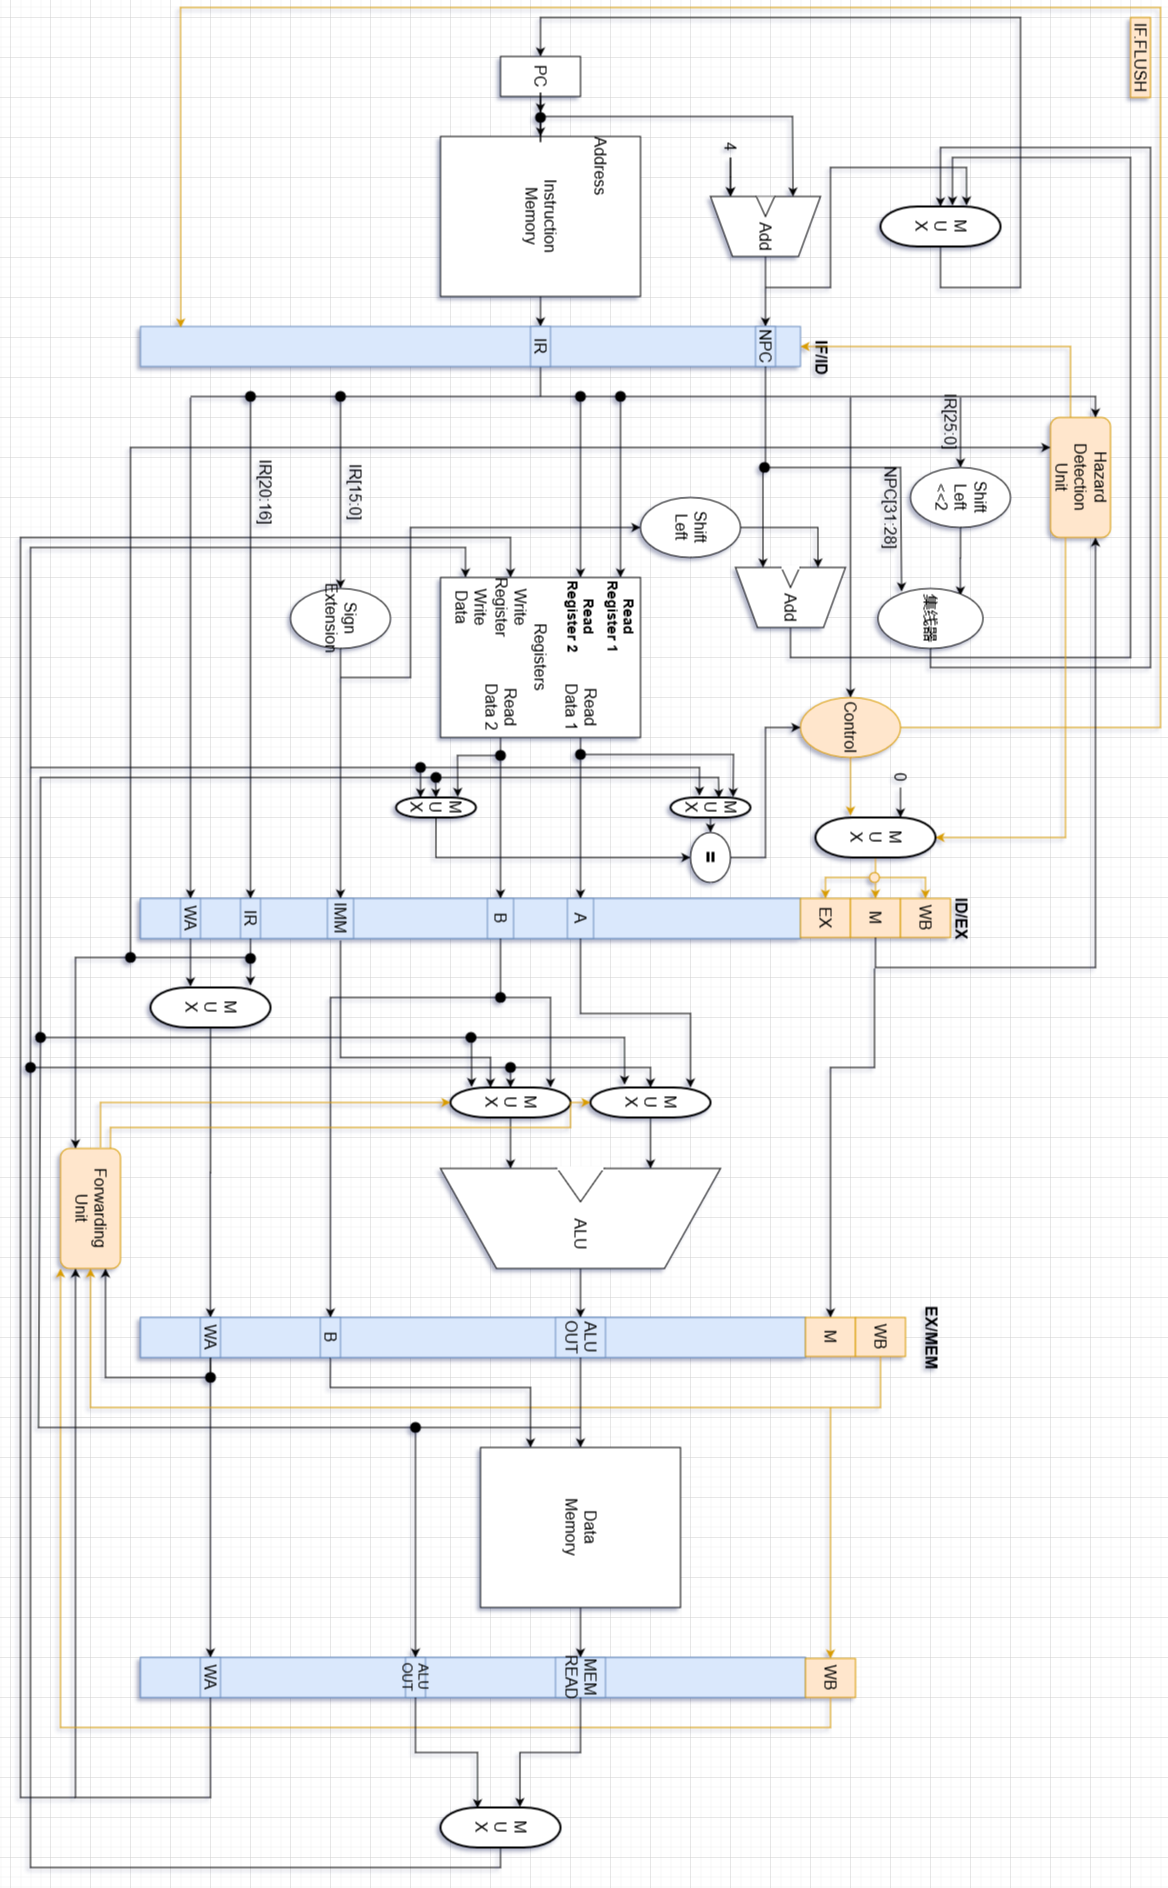
\includegraphics[width=\linewidth*6/7]{data_path.png}
	\label{data_path}
\end{figure}
这个数据通路比较复杂, 花了不少时间来画. 相比于老师给出的数据通路, 里面多了
\begin{itemize}
	\item 一些必要的转发(如给ID段BEQ判等的转发等)
	\item ID段加入了J指令(老师的图中没有J指令)
	\item ALU操作数的MUX加入了对IMM的处理
	\item ...
\end{itemize}
其余内容大多和老师的相似.
\subsection{状态转换}
这里的状态转换主要是PC的转换以及分支预测失误时的指令清空. 指令清空比较简单, 只需要把对应段间寄存器置零即可. 而PC的状态转换主要是这样的:
\begin{figure}[H]
	\centering
	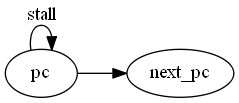
\includegraphics[width=\linewidth/3]{phase_diagram.png}
\end{figure}
也就是, 当需要流水线停顿的时候, 需要禁止PC的更新(当然, 也要置空ID\_EX段, 图中没有呈现)
\subsection{代码讲解}
首先声明, 由于实验要求中, 并不要求写DBU的代码(不过我写了, 可见附件代码), 因此报告中就不加以描述了.\par
流水线CPU比单周期的多周期的CPU要复杂得多, 它的代码模块也比较多, 大体可以分为以下这几类来讲解:
\begin{itemize}
	\item 数据通路的连接
	\item 控制单元的设计
	\item 转发单元(Forwarding Unit)
	\item 冒险探测器
	\item ALU单元*
	\item 寄存器文件*
\end{itemize}
其中, 标*的模块已经在单周期和多周期甚至更早的实验中就已经讲解过多次, 这里再赘述就浪费篇幅了, 因此略去. 主要讲解的代码部分为数据通路, 控制单元, 转发单元, 冒险探测器.
\subsubsection{数据通路代码}
限于篇幅, 就不将所有代码放出来(若有需要, 可查看附件中的代码), 只放一些关键代码.
而关键代码中, 大部分都是按照前述数据通路图(见\ref{data_path}), 这一部分只是简单地用wire变量进行连线, 比较简单. 主要提一下的就是各种数据线的src(source)的相关控制:
\begin{enumerate}
	\item pc\_src(pc soource)的数据通路\\
	会看到,这里对于PC的source有比较多的选择, 这是因为需要考虑分支预测的成功与失败, 各类PC来源等等. 因此看起来比较复杂.
	\begin{lstlisting}[language=verilog]
register_syn #(.N(32)) 
    rIF_ID_NPC(.clk(clk),
               .rst(rst || (flush && ~stall)),
               .we(~stall),
               .wd(PC+4),
               .d(IF_ID_NPC));

//// 跳转指令等的PC赋值
always @(posedge clk, posedge rst) begin
    if(rst) begin
        PC <= 32'h0000_0000;
    end
    else begin
        if(pc_we == 1'b1) begin
            case(pc_src)
                3'b000: PC <= PC + 4;
                3'b001: PC <= IF_ID_NPC + (ID_instr_imm << 2);
                3'b010: PC <= {IF_ID_NPC[31: 28], ID_instr_25_0_sll_2};
                3'b011: PC <= PC;
                3'b100: PC <= PC + 4 + (im_instr_imm << 2);
                3'b101: PC <= IF_ID_NPC;
                default: PC <= PC;
            endcase
        end
        else PC <= PC;
    end
end
	\end{lstlisting}
	\item alu\_src和write\_date\_src的数据通路\\
	这部分和转发单元一起发挥作用, 保证ALU和Data Memory的输入正确.
	\begin{lstlisting}[language=verilog]
always @(*) begin
    case(alu_a_src)
        2'b00: alu_a = ID_EX_A;
        2'b10: alu_a = WB_wb_data;
        2'b11: alu_a = EX_MEM_Y;
        default: alu_a = ID_EX_A;
    endcase
    case(alu_b_src)
        2'b00: alu_b = ID_EX_B;
        2'b01: alu_b = ID_EX_IMM;
        2'b10: alu_b = WB_wb_data;
        2'b11: alu_b = EX_MEM_Y;
        default: alu_b = ID_EX_B;
    endcase
    case(write_data_src)
        2'b00: write_data = ID_EX_B;
        2'b10: write_data = WB_wb_data;
        2'b11: write_data = EX_MEM_Y;
        default: write_data = ID_EX_B;
    endcase
end
	\end{lstlisting}
\end{enumerate}
\subsubsection{控制单元代码}
这里就不展示模块头等了, 直接上重要部分代码:
\begin{enumerate}
	\item pc\_src的处理
	因为设计了思考题中的分支预测, 所以这里的pc\_src还比较复杂, 需要考虑的变量包括但不限于
	\begin{itemize}
		\item 当前是否是分支指令, 如果是, 是beq还是jump
		\item 分支预测的结果是跳转还是不跳转
		\item 现在看来结果应该是跳转还是不跳转
		\item ...
	\end{itemize}
	代码如下,
	\begin{lstlisting}[language=verilog]
always @(*) begin
    if(opcode == BEQ_op) begin
        if(equal) begin
            if(had_branched) begin
                flush = 1'b0;
                if(shall_branch) begin
                    pc_src = 3'b100;
                end
                else begin
                    pc_src = 3'b000;
                end
            end
            else begin
                pc_src = 3'b001;
                flush = 1'b1;
            end
        end
        else begin
            if(had_branched) begin
                flush = 1'b1;
                pc_src = 3'b101;
            end
            else begin
                flush = 1'b0;
                if(shall_branch) begin
                    pc_src = 3'b100;
                end
                else begin
                    pc_src = 3'b000;
                end
            end
        end
    end
    else if(shall_branch) begin
        pc_src = 3'b100;
        flush = 1'b0;
    end
    else if(opcode == J_op) begin
        pc_src = 3'b010;
        flush = 1'b1;
    end
    else begin
        pc_src = 3'b000;
        flush = 1'b0;
    end
end
	\end{lstlisting}
	\item 各种控制信号\\
	这个倒是没什么新奇的, 基本和单周期的一样. 代码如下
	\begin{lstlisting}[language=verilog]
always @(*) begin
    {reg_dst, alu_op, alu_src, mem_read, mem_write, reg_write, mem_to_reg} = 11'h000;
    case(opcode)
        ADD_op: begin
            reg_dst = 1'b1;
            alu_op = 2'b10; // 按 funct
            reg_write = 1'b1;
        end
        ADDI_op: begin
            alu_op = 2'b00; // 做加法
            alu_src = 1'b1; // 选立即数
            reg_write = 1'b1;
        end
        LW_op: begin
            alu_op = 2'b00; // 做加法
            alu_src = 1'b1; // 选立即数
            mem_read = 1'b1;
            reg_write = 1'b1;
            mem_to_reg = 1'b1;
        end
        SW_op: begin
            alu_op = 2'b00; // 做加法
            alu_src = 1'b1; // 选立即数
            mem_write = 1'b1;
        end
        BEQ_op: begin
            alu_src = 1'b1;
        end
        J_op: begin
            alu_src = 1'b1;
        end
        default: {reg_dst, alu_op, alu_src, mem_read, mem_write, reg_write, mem_to_reg} = 11'h000;
    endcase
end
	\end{lstlisting}
\end{enumerate}
\subsubsection{转发单元代码}
转发单元主要是alu\_src的转发, equal\_src的转发, 和write\_data\_src的转发.
\begin{enumerate}
	\item alu\_src的转发\\
	这里alu\_a和alu\_b基本一样, 限于篇幅, 展示alu\_b的(因为它还多了个imm的选择)
	\begin{lstlisting}[language=verilog]
// alu\_b\_src
if(alu_src == 1'b1) begin
    alu_b_src = 2'b01;
end
else if(EX_MEM_WA == ID_EX_rt && EX_MEM_reg_write == 1'b1 && EX_MEM_WA != 5'b00000) begin
    alu_b_src = 2'b11;
end
else if(MEM_WB_WA == ID_EX_rt && MEM_WB_reg_write == 1'b1 && MEM_WB_WA != 5'b00000) begin
    alu_b_src = 2'b10;
end
else begin
    alu_b_src = 2'b00;
end
	\end{lstlisting}
	\item equal\_src的转发\\
	来源有寄存器堆, alu\_y, memory读出结果, EX.MEM段的Y. 代码如下:
	\begin{lstlisting}[language=verilog]
// equal\_a\_src
if(ID_EX_WA == IF_ID_IR[25:21] && ID_EX_reg_write == 1'b1 && ID_EX_WA != 5'b00000) begin
    equal_a_src = 2'b01;
end
else if(EX_MEM_WA == IF_ID_IR[25:21] && EX_MEM_reg_write == 1'b1 && EX_MEM_WA != 5'b00000) begin
    if(EX_MEM_mem_read) begin
        equal_a_src = 2'b10;
    end
    else begin
        equal_a_src = 2'b11;
    end
end
else begin
    equal_a_src = 2'b00;
end
	\end{lstlisting}
	\item write\_data\_src的转发\\
	来源有ID.EX的B, WB段的写回数据, EX.MEM段的Y. 代码如下:
	\begin{lstlisting}[language=verilog]
// write\_data\_src
if(EX_MEM_WA == ID_EX_rt && EX_MEM_reg_write == 1'b1 && EX_MEM_WA != 5'b00000) begin
    write_data_src = 2'b11;
end
else if(MEM_WB_WA == ID_EX_rt && MEM_WB_reg_write == 1'b1 && MEM_WB_WA != 5'b00000) begin
    write_data_src = 2'b10;
end
else begin
    write_data_src = 2'b00;
end
	\end{lstlisting}
\end{enumerate}
\subsubsection{冒险探测器代码}
这一部分主要是为了lw指令(就实验要求的6条指令而言)准备的, 因为它在MEM段才出数据. 代码如下, 在判断到冒险的时候就置stall为1'b1, pc\_we为1'b0即可.
\begin{lstlisting}[language=verilog]
module hazard_detection_unit
(
input mem_read,
input [31:0] IF_ID_IR,
input [31:0] ID_EX_IR,
output reg pc_we,
output reg stall
);

always @(*) begin
    if(mem_read == 1'b1 
        && (ID_EX_IR[20:16] == IF_ID_IR[25:21] 
            || ID_EX_IR[20:16] == IF_ID_IR[20:16])) begin
        pc_we = 1'b0;
        stall = 1'b1;
    end
    else begin
        pc_we = 1'b1;
        stall = 1'b0;
    end
end    
    
endmodule
\end{lstlisting}

\section{实验结果}
再次声明, 由于实验不要求实现DBU, 实验结果就不展示DBU模块了.\par
这次使用的测试代码是助教给出的第二个测试代码(见附录\ref{asm}或提交的代码附件)\par
下面分部分展示仿真结果(花花绿绿的不是出错, 只是这样方便观察流水线各段):
\subsection{start, test0, next0三个部分}
见下图, 可以看到
\begin{enumerate}
	\item 红色框和箭头标识的部分是跳转指令, 都有相应的flush操作
	\item 绿色大框标识了输入给ALU的a,b, 以及ALU的输出y. 都是正确的. 这还说明了转发机制是足够完整的.
	\item 浅蓝色箭头标志了信号或指令的流水线一级一级往下传.
\end{enumerate}
\begin{figure}[H]
	\centering
	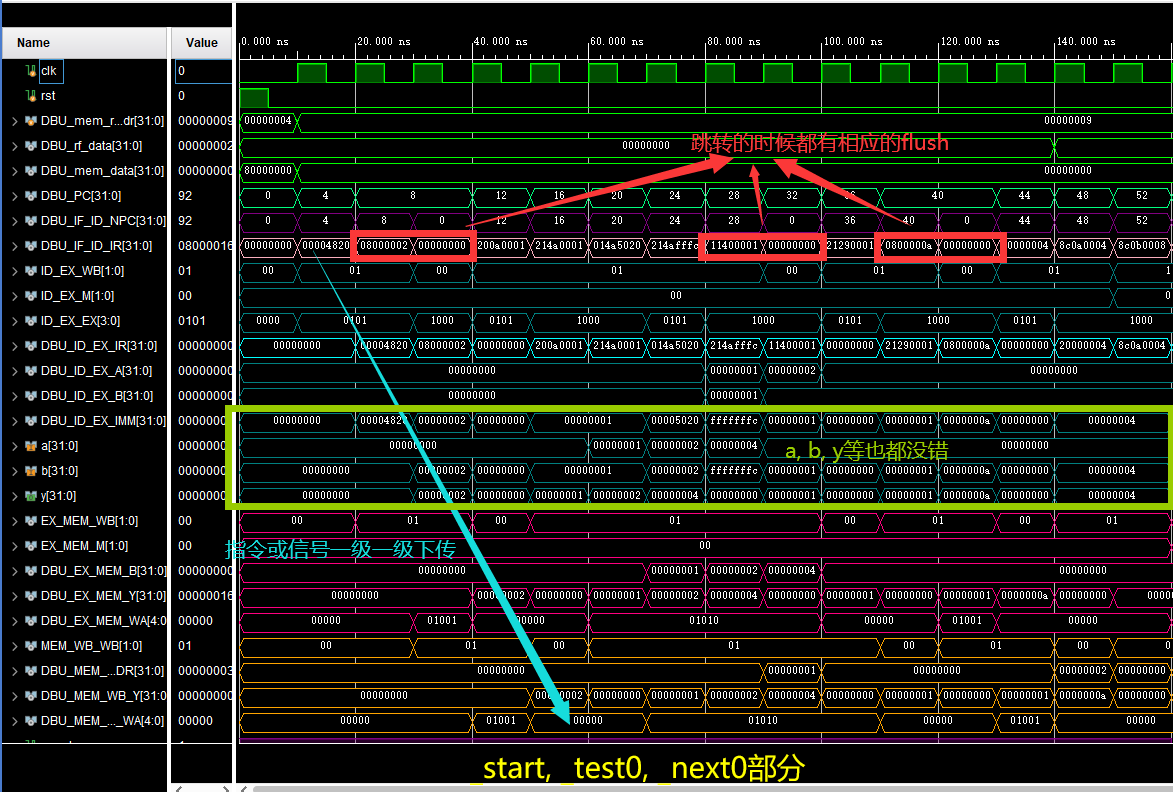
\includegraphics[width=\linewidth]{start_test0_next0.png}
\end{figure}
\subsection{test1, next1, success三个部分}
见下图, 可以看到
\begin{enumerate}
	\item 红色箭头标识了最终结果的正确性, 也就是\$t1=2
	\item 浅蓝色箭头标志了由于LW指令而产生了相关, 因此需要stall, 停顿流水线
\end{enumerate}
\begin{figure}[H]
	\centering
	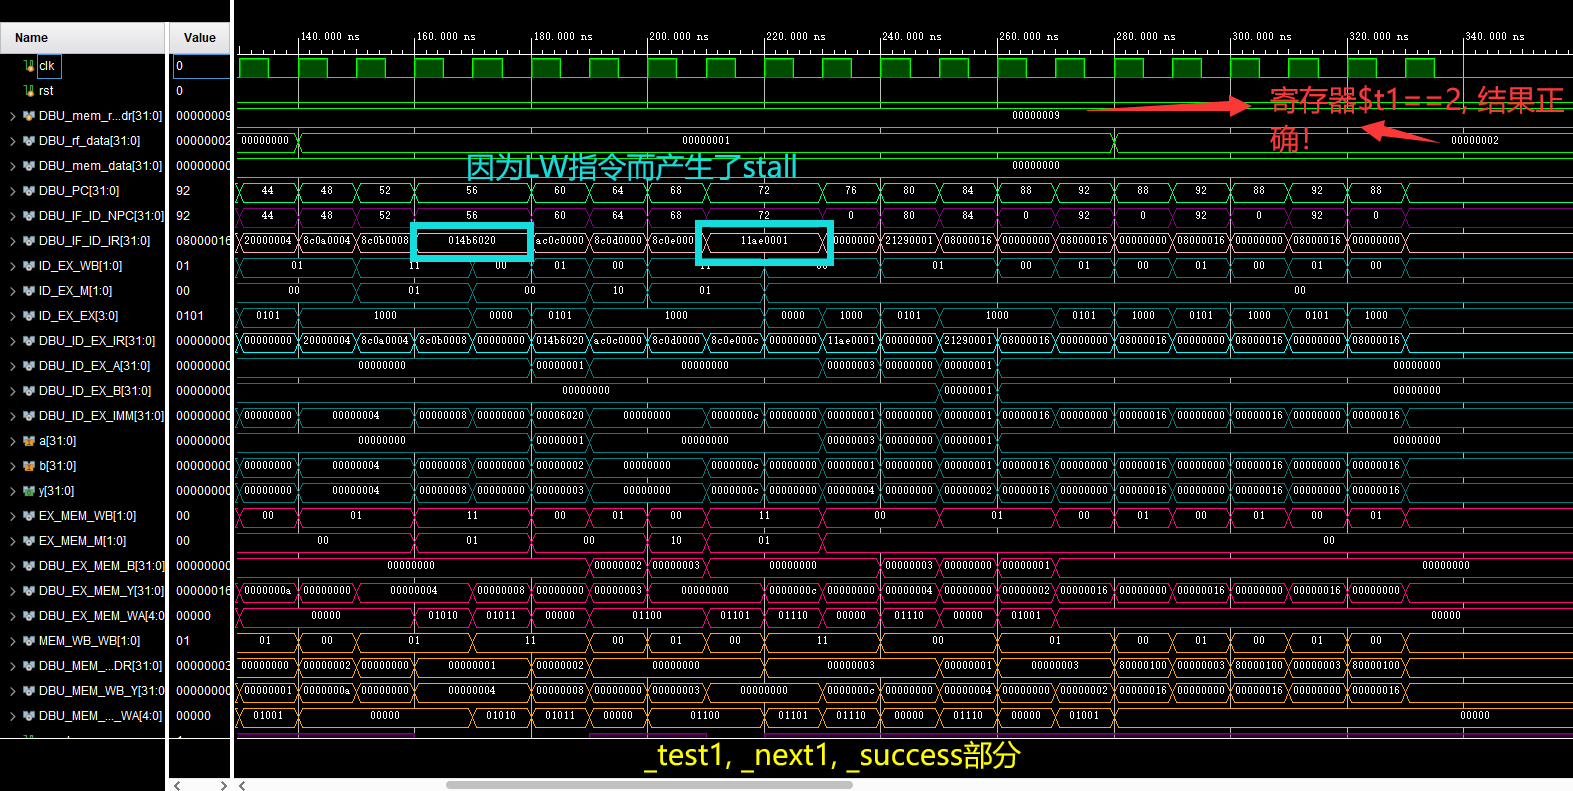
\includegraphics[width=\linewidth]{test1_next1_success.png}
\end{figure}

\section{思考题}
这次思考题要求实现分支预测器.\par
我实现的分支预测器是一个简单的二位动态分支预测.\par
事实上, 前面的讲的代码就是使用了分支预测器的, 只不过默认不跳转, 所以表现出来和没有分支预测器没有任何区别.\par
下面用一个能表现出区别的示例代码(见附录\ref{asm_predictor}\footnote{特别感谢黄致远同学提供测试代码})来展现.\par
\begin{figure}[H]
	\centering
	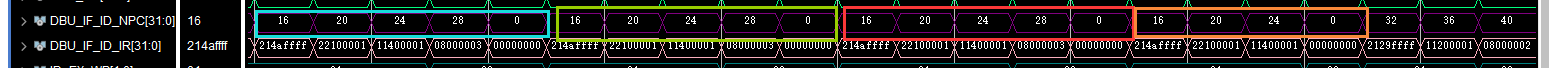
\includegraphics[width=\linewidth]{predictor.png}
\end{figure}
可以看到图中原来一个循环中IF.ID\_NPC是要经历16,20,24,28,0的循环, 过了几次后, 变成16,20,24,0了.\par
反过来也是可以的, 但是限于篇幅就不展示了, 助教如果感兴趣可以自己运行一下我的代码(附件里都有)

\section{心得体会}
本次流水线设计是目前最难的实验了. 除了前面提到的这种, 在ID段做BEQ的方法, 我还尝试了在MEM段做BEQ的方法, 在IF段做Jump的方法等. 均有实现. 但综合考虑, 似乎在ID段做BEQ能权衡好关键路径的长度等问题.\par
此外, 还巩固了分支预测的知识, 并且实现了它.

\section{意见建议}
流水线的数据通路示例比较不完整了, 需要自己补全很多东西. 可以稍微完整一点.

\section{附录}
\subsection{附录1}
\begin{figure}[H]
	\centering
	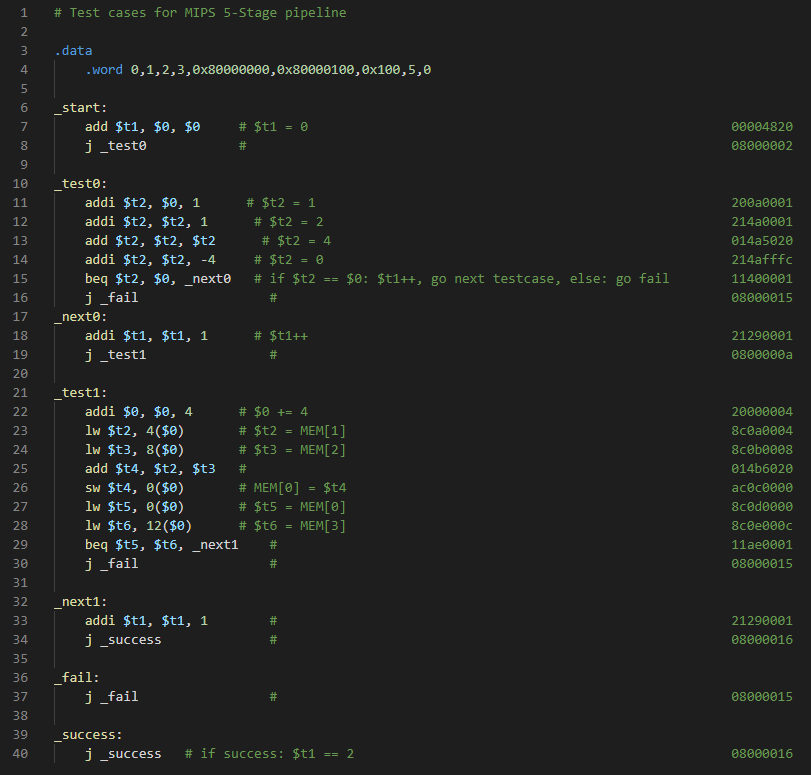
\includegraphics[width=\linewidth]{asm.png}
	\label{asm}
\end{figure}
\subsection{附录2}
\begin{figure}[H]
	\centering
	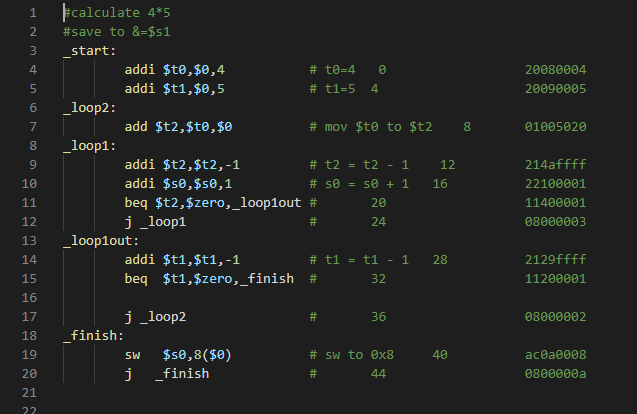
\includegraphics[width=\linewidth]{asm_predictor.png}
	\label{asm_predictor}
\end{figure}


\end{document}






